\documentclass[12pt,a4paper]{article}

\usepackage[a4paper,text={16.5cm,25.2cm},centering]{geometry}
\usepackage{lmodern}
\usepackage{amssymb,amsmath}
\usepackage{bm}
\usepackage{graphicx}
\usepackage{microtype}
\usepackage{hyperref}
\setlength{\parindent}{0pt}
\setlength{\parskip}{1.2ex}

\hypersetup
       {   pdfauthor = {  },
           pdftitle={  },
           colorlinks=TRUE,
           linkcolor=black,
           citecolor=blue,
           urlcolor=blue
       }




\usepackage{upquote}
\usepackage{listings}
\usepackage{xcolor}
\lstset{
    basicstyle=\ttfamily\footnotesize,
    upquote=true,
    breaklines=true,
    breakindent=0pt,
    keepspaces=true,
    showspaces=false,
    columns=fullflexible,
    showtabs=false,
    showstringspaces=false,
    escapeinside={(*@}{@*)},
    extendedchars=true,
}
\newcommand{\HLJLt}[1]{#1}
\newcommand{\HLJLw}[1]{#1}
\newcommand{\HLJLe}[1]{#1}
\newcommand{\HLJLeB}[1]{#1}
\newcommand{\HLJLo}[1]{#1}
\newcommand{\HLJLk}[1]{\textcolor[RGB]{148,91,176}{\textbf{#1}}}
\newcommand{\HLJLkc}[1]{\textcolor[RGB]{59,151,46}{\textit{#1}}}
\newcommand{\HLJLkd}[1]{\textcolor[RGB]{214,102,97}{\textit{#1}}}
\newcommand{\HLJLkn}[1]{\textcolor[RGB]{148,91,176}{\textbf{#1}}}
\newcommand{\HLJLkp}[1]{\textcolor[RGB]{148,91,176}{\textbf{#1}}}
\newcommand{\HLJLkr}[1]{\textcolor[RGB]{148,91,176}{\textbf{#1}}}
\newcommand{\HLJLkt}[1]{\textcolor[RGB]{148,91,176}{\textbf{#1}}}
\newcommand{\HLJLn}[1]{#1}
\newcommand{\HLJLna}[1]{#1}
\newcommand{\HLJLnb}[1]{#1}
\newcommand{\HLJLnbp}[1]{#1}
\newcommand{\HLJLnc}[1]{#1}
\newcommand{\HLJLncB}[1]{#1}
\newcommand{\HLJLnd}[1]{\textcolor[RGB]{214,102,97}{#1}}
\newcommand{\HLJLne}[1]{#1}
\newcommand{\HLJLneB}[1]{#1}
\newcommand{\HLJLnf}[1]{\textcolor[RGB]{66,102,213}{#1}}
\newcommand{\HLJLnfm}[1]{\textcolor[RGB]{66,102,213}{#1}}
\newcommand{\HLJLnp}[1]{#1}
\newcommand{\HLJLnl}[1]{#1}
\newcommand{\HLJLnn}[1]{#1}
\newcommand{\HLJLno}[1]{#1}
\newcommand{\HLJLnt}[1]{#1}
\newcommand{\HLJLnv}[1]{#1}
\newcommand{\HLJLnvc}[1]{#1}
\newcommand{\HLJLnvg}[1]{#1}
\newcommand{\HLJLnvi}[1]{#1}
\newcommand{\HLJLnvm}[1]{#1}
\newcommand{\HLJLl}[1]{#1}
\newcommand{\HLJLld}[1]{\textcolor[RGB]{148,91,176}{\textit{#1}}}
\newcommand{\HLJLs}[1]{\textcolor[RGB]{201,61,57}{#1}}
\newcommand{\HLJLsa}[1]{\textcolor[RGB]{201,61,57}{#1}}
\newcommand{\HLJLsb}[1]{\textcolor[RGB]{201,61,57}{#1}}
\newcommand{\HLJLsc}[1]{\textcolor[RGB]{201,61,57}{#1}}
\newcommand{\HLJLsd}[1]{\textcolor[RGB]{201,61,57}{#1}}
\newcommand{\HLJLsdB}[1]{\textcolor[RGB]{201,61,57}{#1}}
\newcommand{\HLJLsdC}[1]{\textcolor[RGB]{201,61,57}{#1}}
\newcommand{\HLJLse}[1]{\textcolor[RGB]{59,151,46}{#1}}
\newcommand{\HLJLsh}[1]{\textcolor[RGB]{201,61,57}{#1}}
\newcommand{\HLJLsi}[1]{#1}
\newcommand{\HLJLso}[1]{\textcolor[RGB]{201,61,57}{#1}}
\newcommand{\HLJLsr}[1]{\textcolor[RGB]{201,61,57}{#1}}
\newcommand{\HLJLss}[1]{\textcolor[RGB]{201,61,57}{#1}}
\newcommand{\HLJLssB}[1]{\textcolor[RGB]{201,61,57}{#1}}
\newcommand{\HLJLnB}[1]{\textcolor[RGB]{59,151,46}{#1}}
\newcommand{\HLJLnbB}[1]{\textcolor[RGB]{59,151,46}{#1}}
\newcommand{\HLJLnfB}[1]{\textcolor[RGB]{59,151,46}{#1}}
\newcommand{\HLJLnh}[1]{\textcolor[RGB]{59,151,46}{#1}}
\newcommand{\HLJLni}[1]{\textcolor[RGB]{59,151,46}{#1}}
\newcommand{\HLJLnil}[1]{\textcolor[RGB]{59,151,46}{#1}}
\newcommand{\HLJLnoB}[1]{\textcolor[RGB]{59,151,46}{#1}}
\newcommand{\HLJLoB}[1]{\textcolor[RGB]{102,102,102}{\textbf{#1}}}
\newcommand{\HLJLow}[1]{\textcolor[RGB]{102,102,102}{\textbf{#1}}}
\newcommand{\HLJLp}[1]{#1}
\newcommand{\HLJLc}[1]{\textcolor[RGB]{153,153,119}{\textit{#1}}}
\newcommand{\HLJLch}[1]{\textcolor[RGB]{153,153,119}{\textit{#1}}}
\newcommand{\HLJLcm}[1]{\textcolor[RGB]{153,153,119}{\textit{#1}}}
\newcommand{\HLJLcp}[1]{\textcolor[RGB]{153,153,119}{\textit{#1}}}
\newcommand{\HLJLcpB}[1]{\textcolor[RGB]{153,153,119}{\textit{#1}}}
\newcommand{\HLJLcs}[1]{\textcolor[RGB]{153,153,119}{\textit{#1}}}
\newcommand{\HLJLcsB}[1]{\textcolor[RGB]{153,153,119}{\textit{#1}}}
\newcommand{\HLJLg}[1]{#1}
\newcommand{\HLJLgd}[1]{#1}
\newcommand{\HLJLge}[1]{#1}
\newcommand{\HLJLgeB}[1]{#1}
\newcommand{\HLJLgh}[1]{#1}
\newcommand{\HLJLgi}[1]{#1}
\newcommand{\HLJLgo}[1]{#1}
\newcommand{\HLJLgp}[1]{#1}
\newcommand{\HLJLgs}[1]{#1}
\newcommand{\HLJLgsB}[1]{#1}
\newcommand{\HLJLgt}[1]{#1}


\begin{document}




\section{Statistics and Benchmarks}
\subsection{Signal to Noise Ratio}
The signal-to-noise ratio calculated in the simulation is a rough estimate. Since the peaks in the Fourier transform seem to be consistently narrow, an arbitrary window is chosen to separate the signal peak from the noise. Signal-to-noise is then calculated by taking the maximum inside each peak window, shifting it downwards by the mean of the noise part, then dividing the resulting value by the variance of the noise part.

\section{Number of Emitting Atoms}


\subsection{Parameters}
\begin{tabular}
{c | c}
Description & Value(s) \\
\hline
mean photon count rate (GHz) & 2.0e6 \\
number of atoms & [10, 20, 30, 40, 50, 60, 70, 80, 90, 100, 200, 500, 800, 1000] \\
randomize each trial & true \\
dead time (ns) & 0.0 \\
resolution (ns) & 0.01 \\
line frequencies (GHz) & [456810, 456813] \\
measurement duration (ns) & 20.0 \\
trials & 100 \\
\end{tabular}
\subsection{Plots}

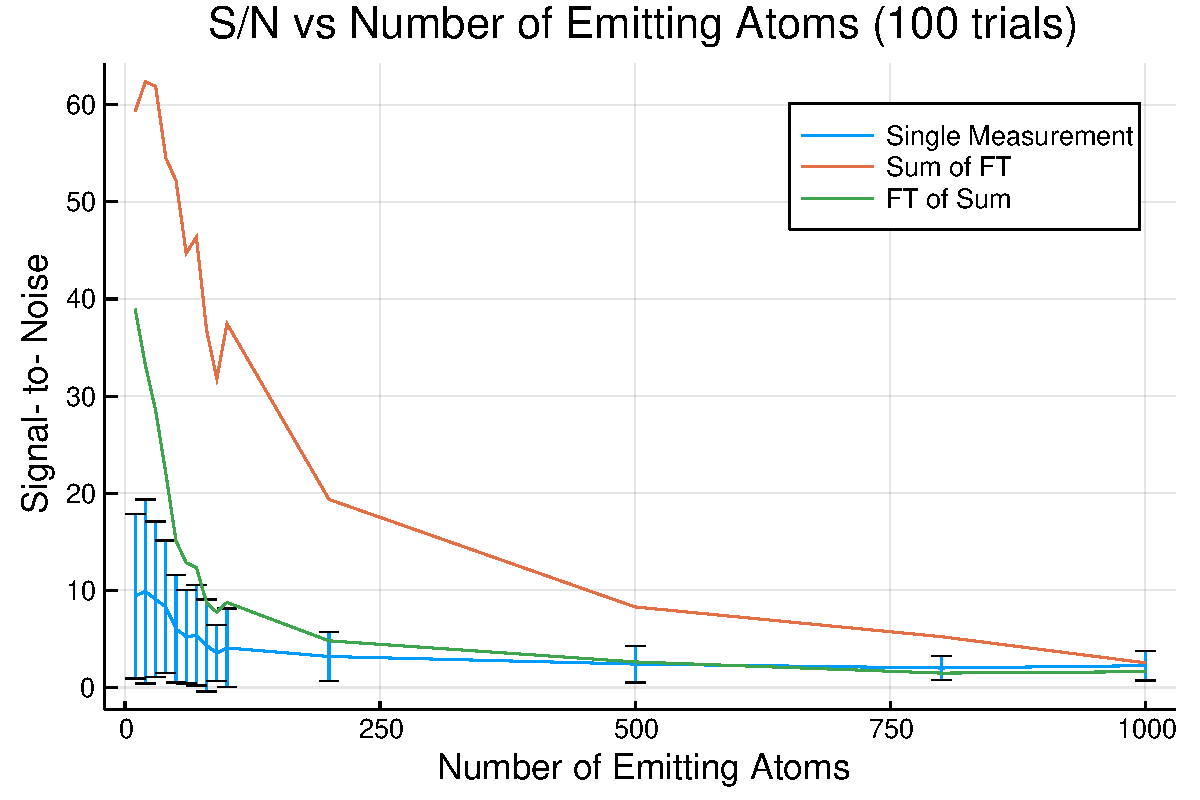
\includegraphics[width=\linewidth]{jl_PKMVtA/simnb_3_1.pdf}

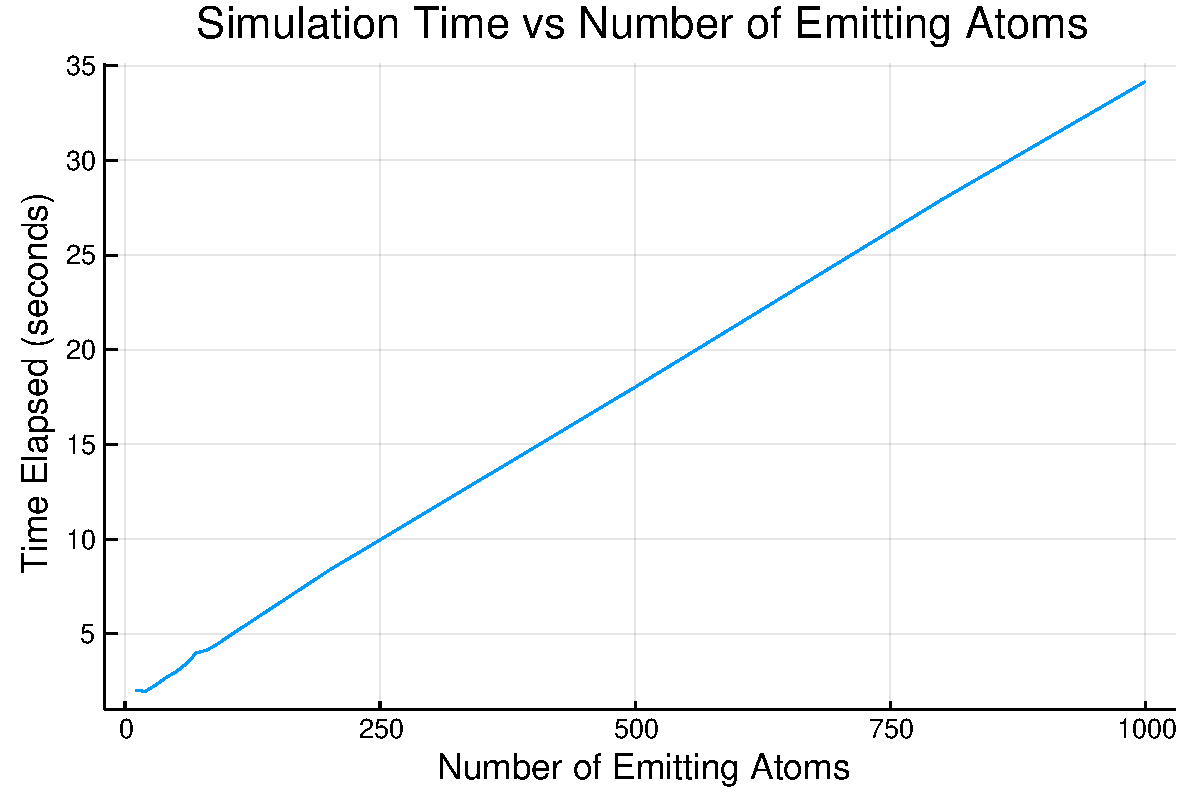
\includegraphics[width=\linewidth]{jl_PKMVtA/simnb_4_1.pdf}

\section{Average Photon Count Rate}


\subsection{Parameters}
\begin{tabular}
{c | c}
Description & Value(s) \\
\hline
mean photon count rate (GHz) & [2.0e6, 200000.0, 20000.0, 2000.0, 200.0, 20.0, 2.0, 0.2] \\
number of atoms & 100 \\
randomize each trial & true \\
dead time (ns) & 0.0 \\
resolution (ns) & 0.01 \\
line frequencies (GHz) & [456810, 456813] \\
measurement duration (ns) & 20.0 \\
trials & 100 \\
\end{tabular}
\subsection{Plots}

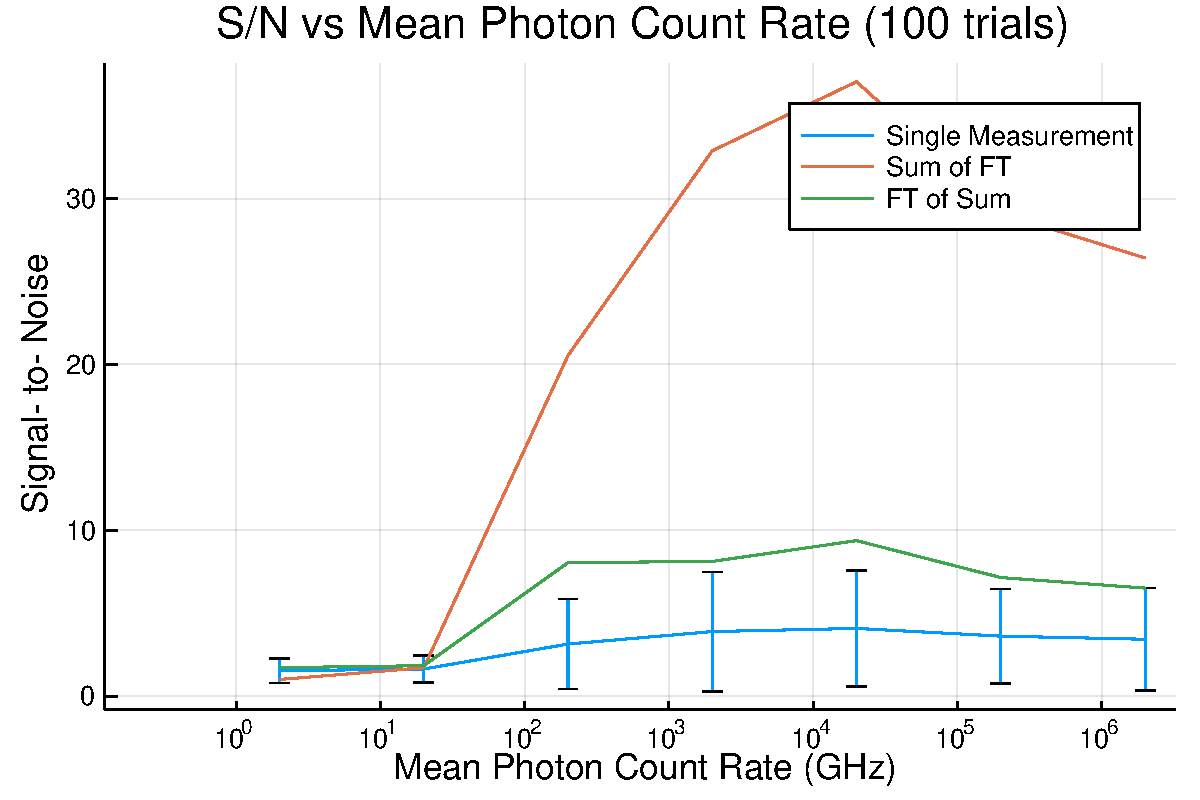
\includegraphics[width=\linewidth]{jl_PKMVtA/simnb_6_1.pdf}

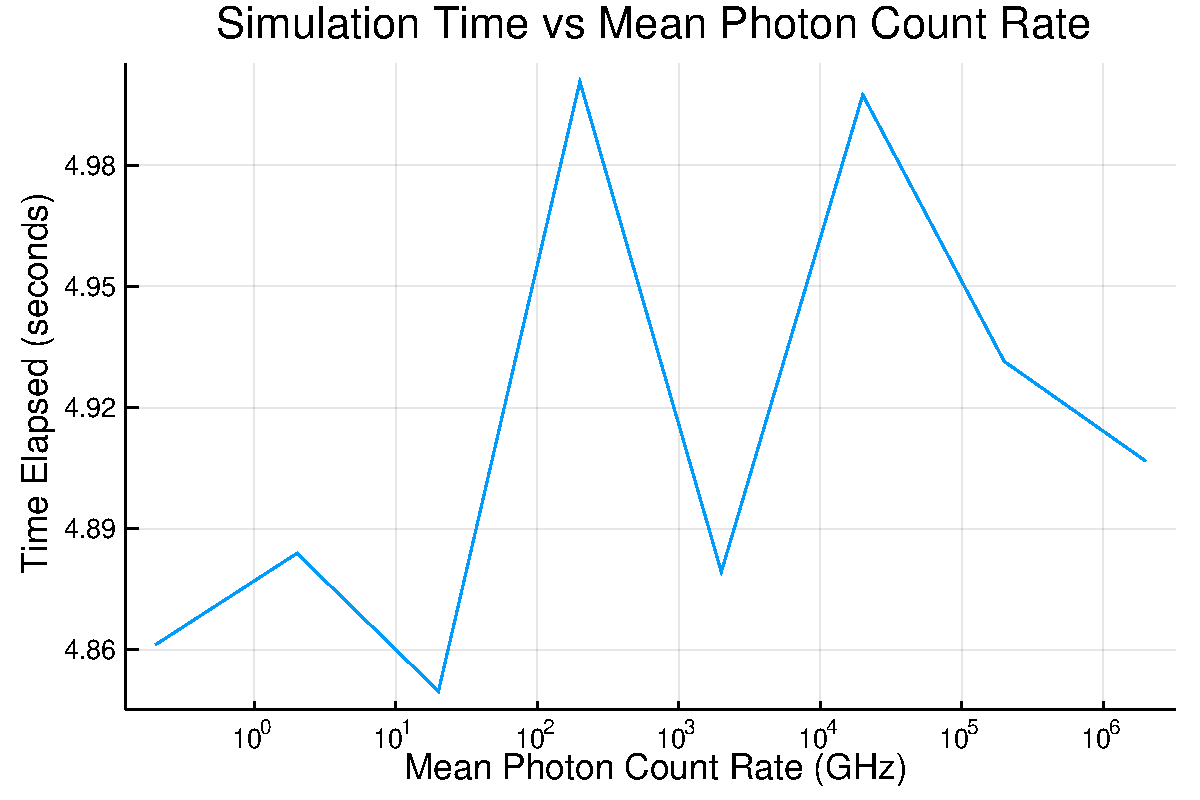
\includegraphics[width=\linewidth]{jl_PKMVtA/simnb_7_1.pdf}

\section{Resolution}


\subsection{Parameters}
\begin{tabular}
{c | c}
Description & Value(s) \\
\hline
mean photon count rate (GHz) & 2.0e6 \\
number of atoms & 100 \\
randomize each trial & true \\
dead time (ns) & 0.0 \\
resolution (ns) & [0.01, 0.02, 0.04, 0.05, 0.06, 0.07, 0.08, 0.09, 0.1] \\
line frequencies (GHz) & [456810, 456813] \\
measurement duration (ns) & 20.0 \\
trials & 100 \\
\end{tabular}
\subsection{Plots}

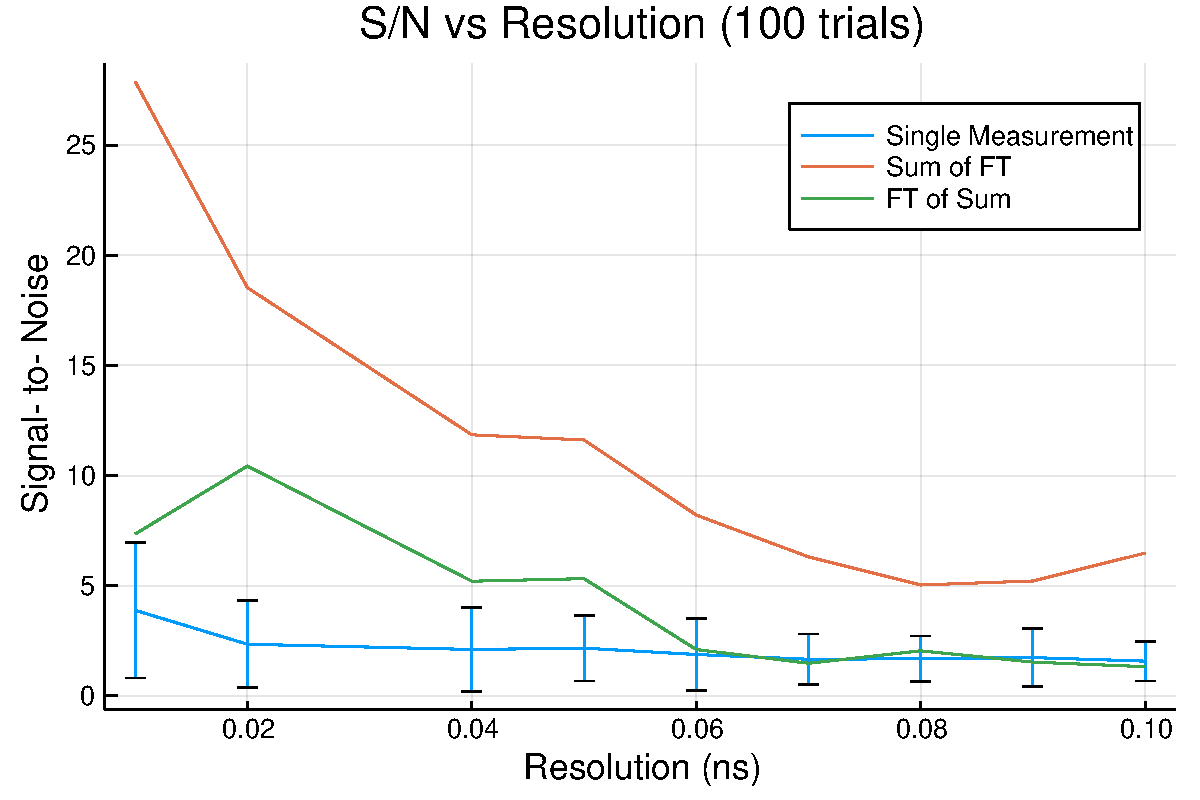
\includegraphics[width=\linewidth]{jl_PKMVtA/simnb_9_1.pdf}

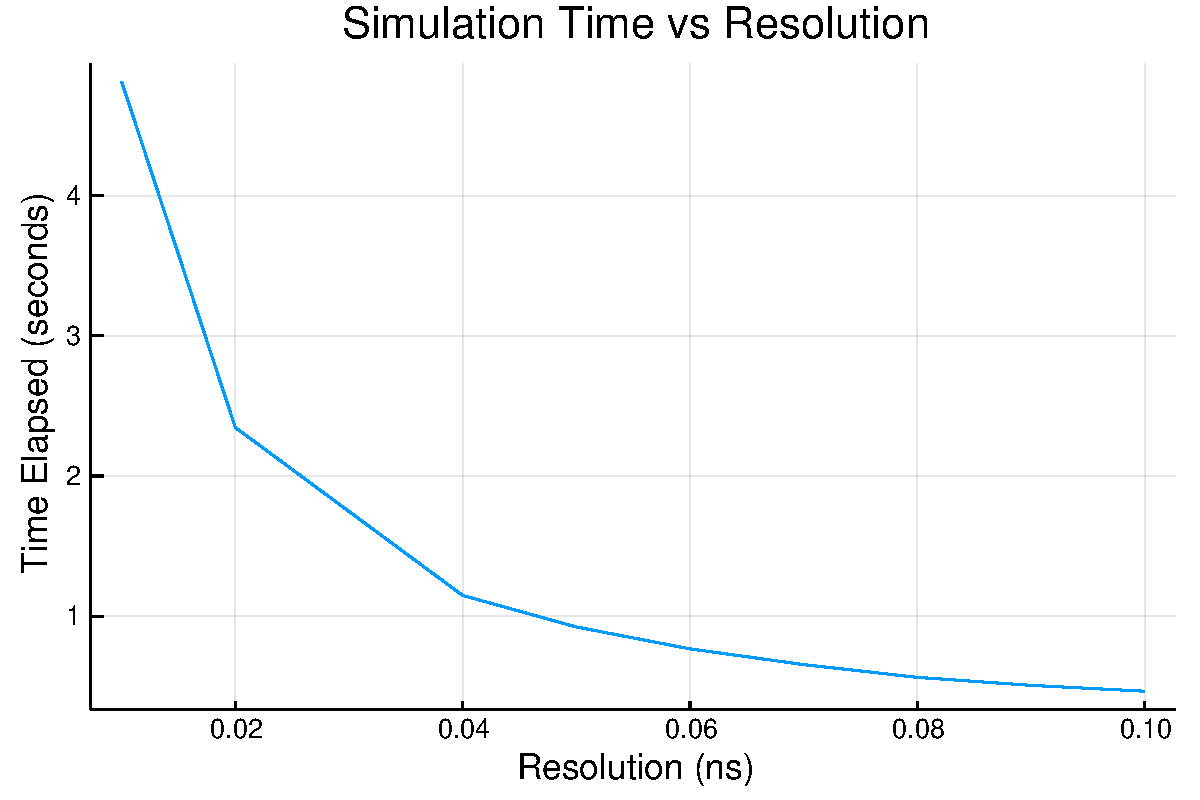
\includegraphics[width=\linewidth]{jl_PKMVtA/simnb_10_1.pdf}

\section{Measurement Duration}
Note: correlation integration time is set to 1/2 the measurement duration for all cases.



\subsection{Parameters}
\begin{tabular}
{c | c}
Description & Value(s) \\
\hline
mean photon count rate (GHz) & 2.0e6 \\
number of atoms & 100 \\
randomize each trial & true \\
dead time (ns) & 0.0 \\
resolution (ns) & 0.01 \\
line frequencies (GHz) & [456810, 456813] \\
measurement duration (ns) & [5.0, 10.0, 15.0, 20.0, 25.0, 30.0, 35.0, 40.0, 45.0, 50.0, 55.0, 60.0, 65.0, 70.0, 75.0, 80.0, 85.0, 90.0, 95.0, 100.0] \\
trials & 100 \\
\end{tabular}
\subsection{Plots}

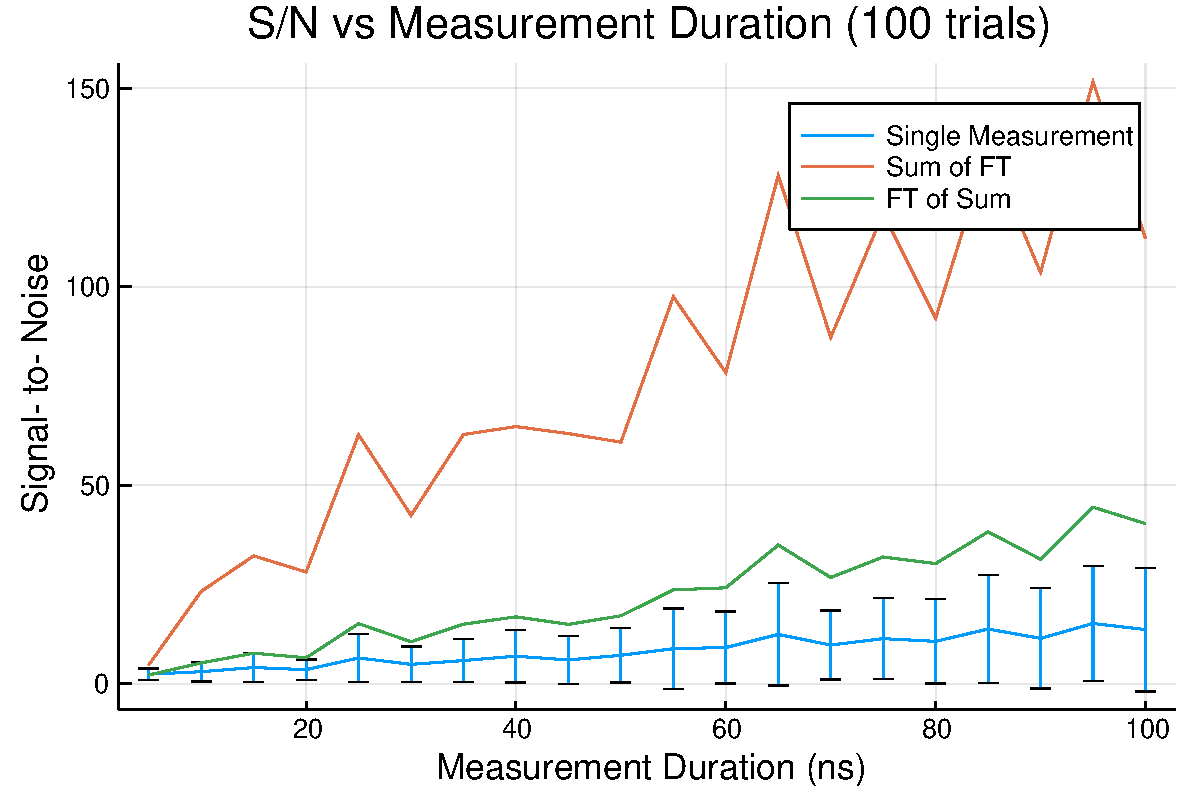
\includegraphics[width=\linewidth]{jl_PKMVtA/simnb_12_1.pdf}

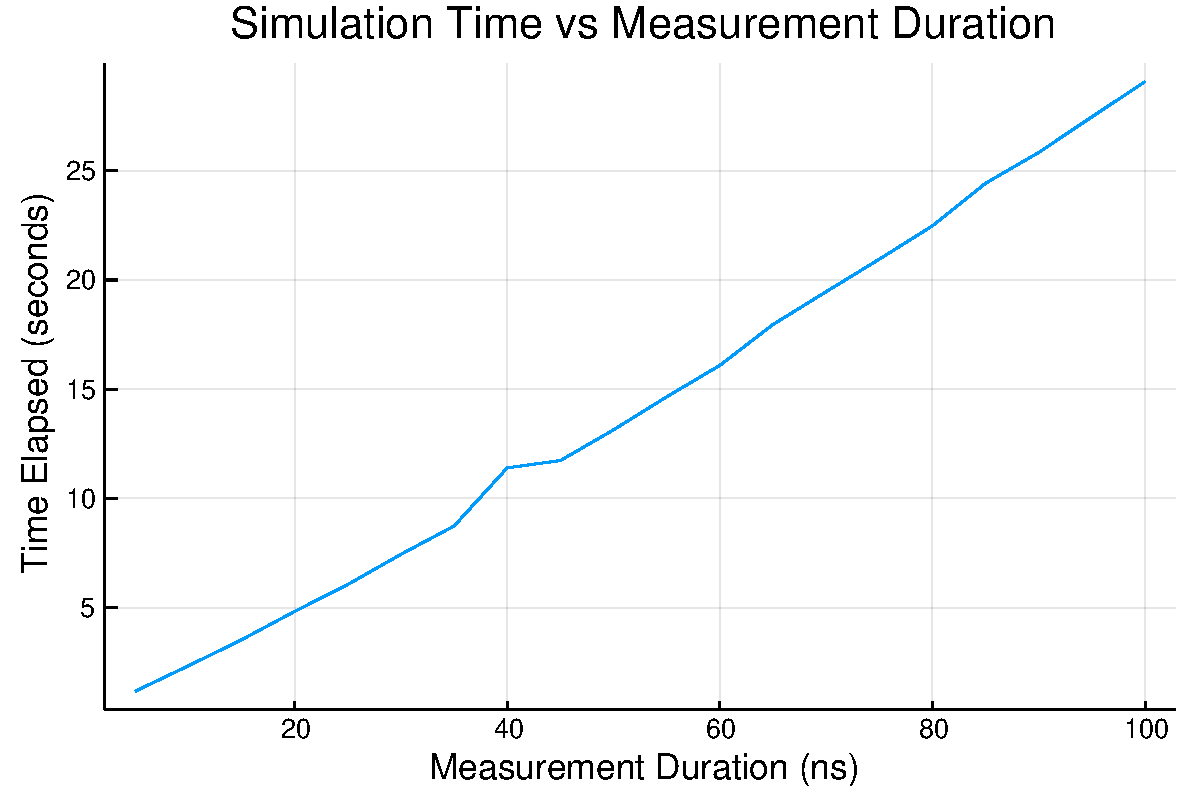
\includegraphics[width=\linewidth]{jl_PKMVtA/simnb_13_1.pdf}

\section{Repeated Measurements}


\subsection{Parameters}
\begin{tabular}
{c | c}
Description & Value(s) \\
\hline
mean photon count rate (GHz) & 2.0e6 \\
number of atoms & 100 \\
randomize each trial & true \\
dead time (ns) & 0.0 \\
resolution (ns) & 0.01 \\
line frequencies (GHz) & [456810, 456813] \\
measurement duration (ns) & 20.0 \\
trials & [10, 20, 30, 40, 50, 60, 70, 80, 90, 100] \\
\end{tabular}
\subsection{Plots}

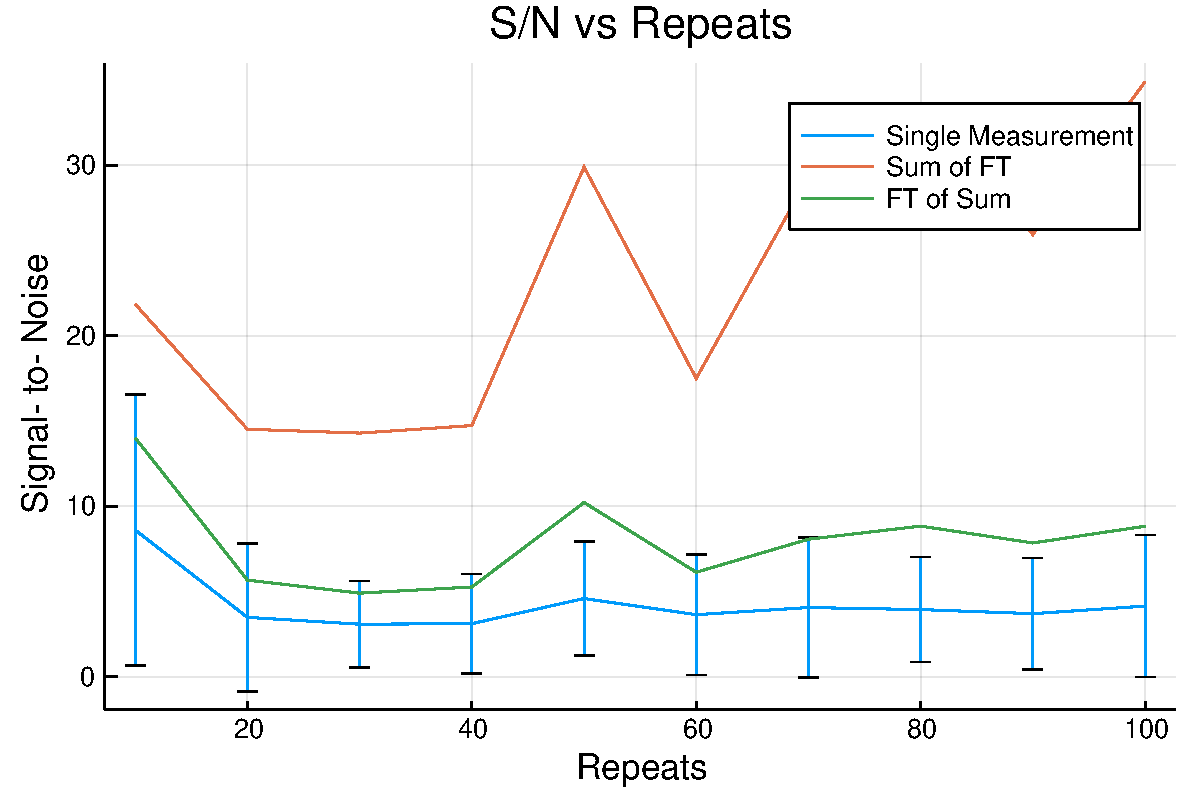
\includegraphics[width=\linewidth]{jl_PKMVtA/simnb_15_1.pdf}

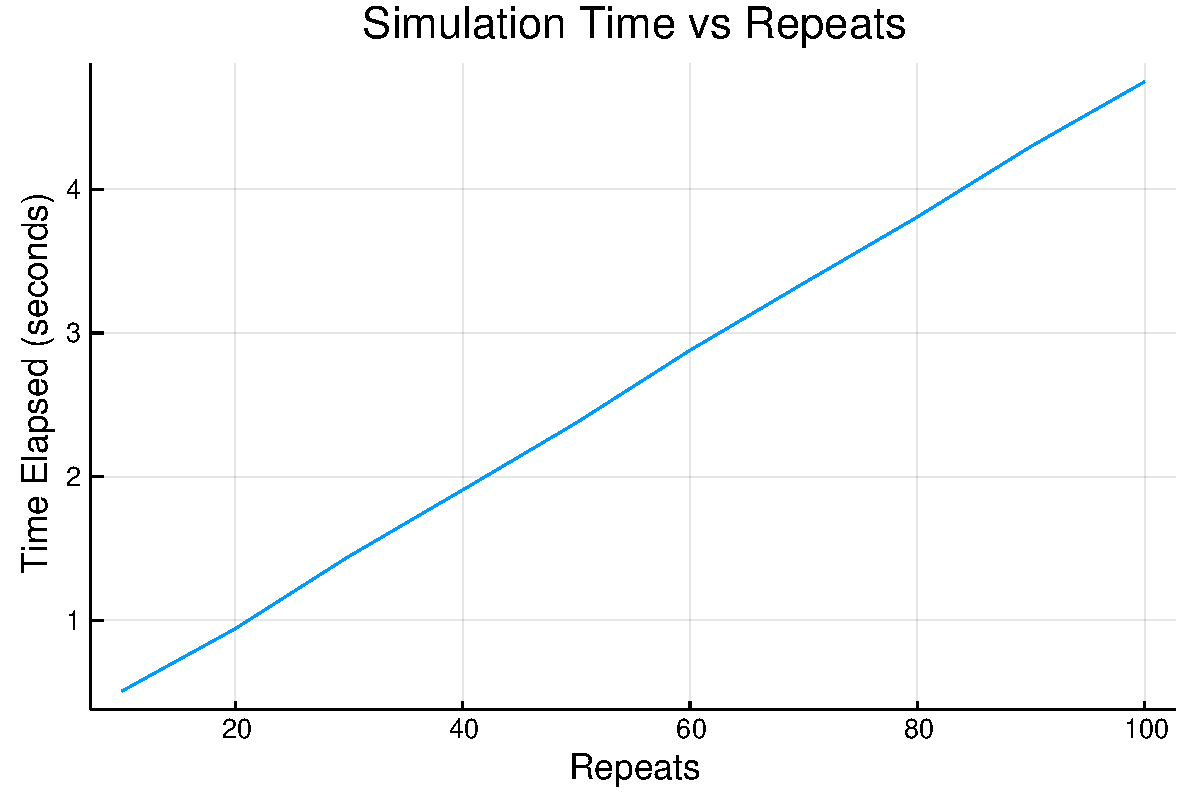
\includegraphics[width=\linewidth]{jl_PKMVtA/simnb_16_1.pdf}


\end{document}
